% Reference snippets; the manuscript embeds these environments directly.
\begin{figure}[t]
\centering
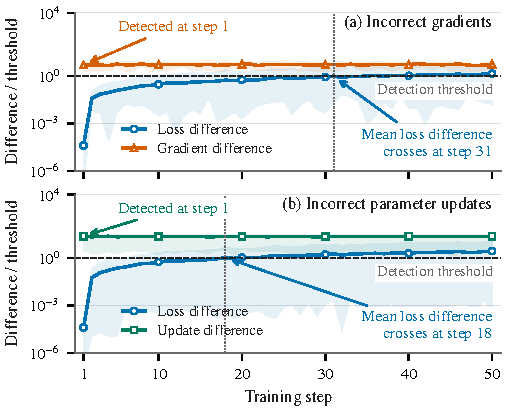
\includegraphics[width=\columnwidth]{figures/gradient_drift.pdf}
\caption{Gradient and update checks detect faults at step~1 in every run; the mean loss difference crosses its threshold at steps 31 and 18 in (a) and (b), respectively. Each panel shows 12 independent training runs. Curves show means and shading shows ranges, normalized by each signal's threshold. The dashed line marks the detection threshold.}
\label{fig:gradient-drift}
\end{figure}

\begin{figure*}[t]
\centering
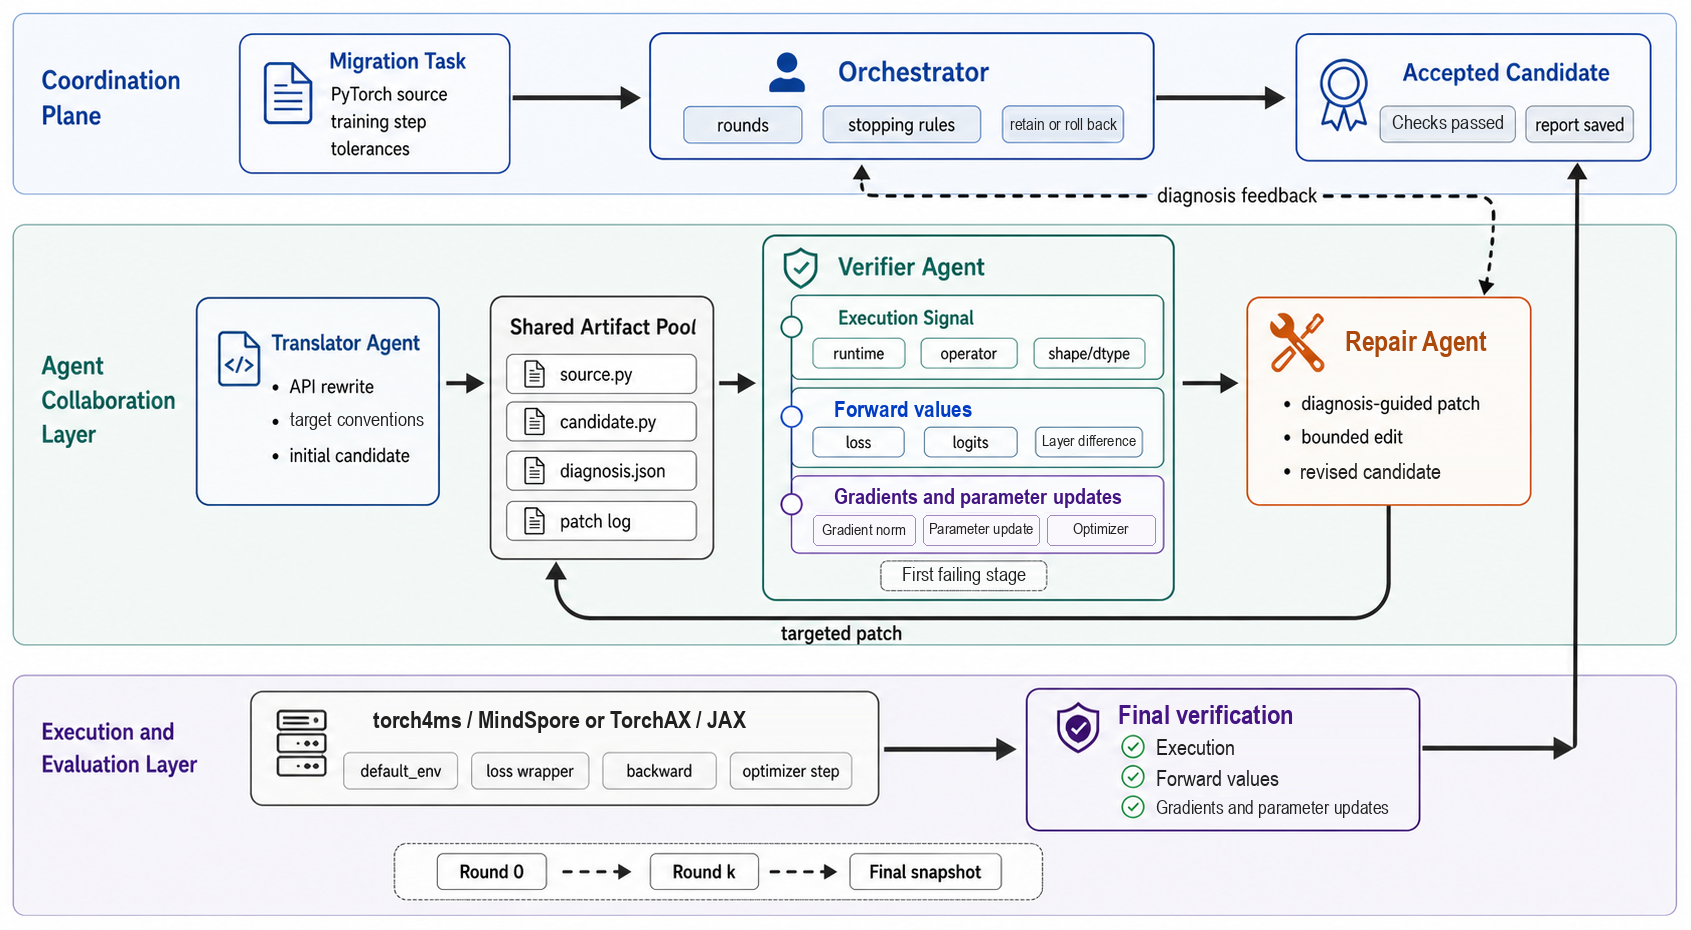
\includegraphics[width=0.97\textwidth]{figures/hierarchical_feedback_architecture.png}
\caption{MARS's repair loop. An orchestrator coordinates the translator, verifier, and repair agents. The verifier's diagnosis guides edits to the permitted code, followed by verification of the updated program. The \texttt{torch4ms}/MindSpore and TorchAX/JAX implementations use the same diagnostic signals and repair procedure.}
\label{fig:architecture}
\end{figure*}

\begin{figure*}[t]
\centering
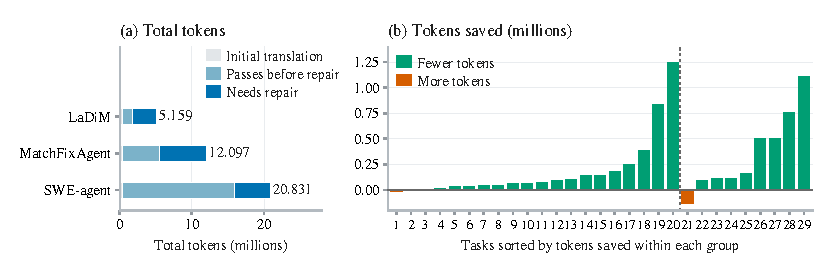
\includegraphics[width=\textwidth]{figures/repair_comparison.pdf}
\caption{Repair cost and acceptance on the 50 MindSpore instances. (a) First-attempt acceptance versus total tokens divided by repairs accepted within four attempts. (b) Cumulative acceptance at the recorded budgets of one, two, and four attempts; connecting lines are visual guides. Methods and acceptance checks follow Tables~\ref{tab:main-results} and~\ref{tab:feedback-ablation}.}
\label{fig:repair-comparison}
\end{figure*}
